After porting, we obtained a valid (meaning, compiling and running) version of BWA processing sequences in batches, originating from GASE-GASAL2.

BWA operates with the seed-extension paradigm, and GASAL2 can run the extension part. For a single query sequence, a variable number of seeds can be found. If we refine this model, the ones located very close to each other are merged and are considered a single entity called chain. For every chain found in the query, a large area is taken in the genome around the chain location in the reference, to make a corresponding target sequence. Its length is around 1.3 times the length of the query sequence. The extension step is then either:

\begin{itemize}
	\item skipped, meaning that the chain is exactly the size of the sequence,
	\item or done only on one side, if the chain is located at the beginning or the end of the query sequence,
	\item or done on both sides, if the chain is in the middle of the sequence.
\end{itemize}

Most of the time, both sides have to be extended. We create then two GPU batches. A simple approach would be to define a batch for the left side, and one for the right side. However, there is a slightly more optimized way to split the alignments between two batches.

We reviewed earlier what thread divergence is. It is more interesting to operate on similar data sets to make the GPU run as many times the same instructions as possible. But if a chain is located on the far left, and another more on the right, knowing that all queries have the same length, the left parts of the extension will have very different lengths, as shown on Figure~\ref{fig:seds-different-chains}. Moreover, the processing time will be limited by the length of its longest alignment. 
\begin{figure}[h!]
	\centering
	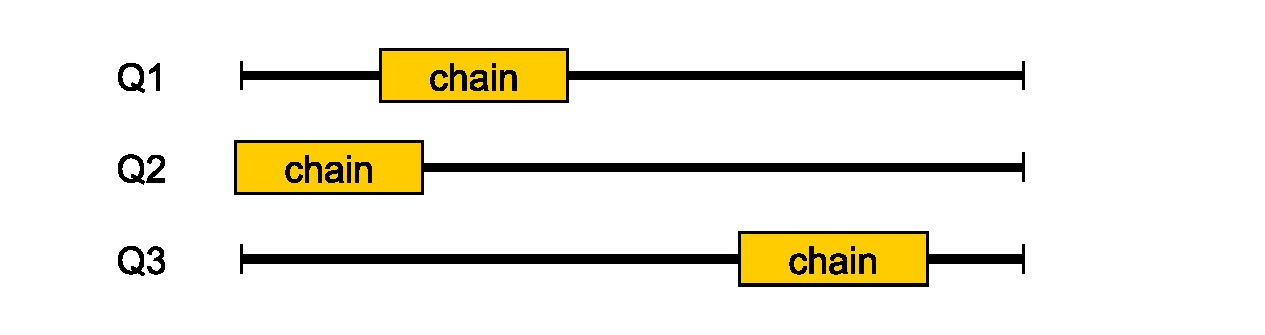
\includegraphics[width=0.7\linewidth]{seds-different-chains}
	\caption{Illustration of chains (in green) being located on different places}
	\label{fig:seds-different-chains}
\end{figure}
To summarize, we note that :
\begin{itemize}
	\item all queries have the same length,
	\item the final score is equal to the sum of the chain score, the left side score, and the right side score,
	\item to that extent, we don't need to know whose score is the left one and the right one (only the sum matters),
	\item and we would like to process both sides in parallel.
\end{itemize}

So instead of using two batches for left and right extension, we use these two batches for long and short extension. This puts the long sides together to minimize thread divergence. The difference between the longest and the shortest extension in each batch is now at most half the length of the query sequence. For each chain, we log in a dedicated data structure if it has zero, one or two alignments, and on which part (left or right) the long alignment is. When both the "long" and "short" batches of extension are done, the scores are gathered.

Another problem arises: since all chains may have only one extension, the short and long batches can have a different number of extension to make. For example, assume that we have three chains as in Figure~\ref{fig:seds-different-chains}. For the sake of conciseness, only queries sequences have been represented, but assume each of these queries have a corresponding target sequence with the same chain located in it, forming pairs of queries-target sequences. Table~\ref{tbl:batches} shows how the batches are filled for this case. Notice how sequences are not aligned together. At the gathering phase, the data structure containing the chain log mentioned above is read to know how many alignments there are for each chain, ensuring proper recollection. Finally, logging how many alignments there is for each chain allow to correct the final score. In BLAST-like paradigm, the scores are computed one after the other, so there is no global recollection like this. Here, we run all the extensions with as starting score the chain score. When gathering the result, if we sum both left and right scores, we count the chain score twice, so we have to subtract the chain score. When only one extension is made (or none), we do not have to do this subtraction.

\begin{table}
	\centering
	\begin{tabular}{|c|c|}
		\hline 
		\textbf{"Long" batch} & \textbf{"Short" batch} \\ 
		\hline 
		Pair 1, right part & Pair 1, left part \\ 
		\hline 
		Pair 2, right part & Pair 3, right part \\ 
		\hline 
		Pair 3, left part &  \\ 
		\hline 
	\end{tabular} 
	\caption{Example of how batches are filled.}
	\label{tbl:batches}
\end{table}

